\documentclass{standalone}
\usepackage{tikz}
\usetikzlibrary{decorations, decorations.text,backgrounds}

\definecolor{CharCoalDark}{RGB}{13, 16, 19}
%% Document
\begin{document}
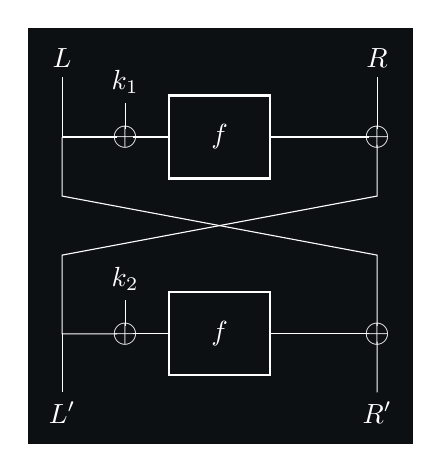
\begin{tikzpicture}[auto,transform shape,background rectangle/.style={fill=CharCoalDark}, show background rectangle]
\tikzstyle{block} = [rectangle, draw, thick,
    text width=3em, text centered, minimum height=3em, color=white]
\tikzstyle{line} = [draw, -]

\node [block] (Et) {$f$};
\coordinate [above of=Et, node distance=1cm] (top);
\coordinate [left of=Et, node distance=2cm] (midleft);
\node [left of=top, node distance=2cm, color=white] (m1) {$L$};
\node [left of=Et, node distance=1.2cm, thick, scale=1.2, color=white] (xor1) {$\mathbf{\oplus}$};
\node [above of=xor1, node distance=0.7cm, color=white] (4L1) {$k_{1}$};
\coordinate [left of=xor1, node distance=1mm] (xor11);
\path [line,color=white] (m1) -- (midleft) -- (xor11);
\coordinate [above of=xor1, node distance=1mm] (xor12);
\path [line, color=white] (4L1) -- (xor12);
\coordinate [right of=xor1, node distance=1mm] (xor13);
\path [line,color=white] (xor13) -- (Et);
%
\node [right of=top, node distance=2cm, color=white] (m2) {$R$};
\node [right of=Et, node distance=2cm, thick, scale=1.2,color=white] (xor2) {$\mathbf{\oplus}$};
\coordinate [left of=xor2, node distance=1mm, color=white] (xor21);
\path [line,color=white] (Et) -- (xor21);
\coordinate [above of=xor2, node distance=1mm,color=white] (xor22);
\path [line,color=white] (m2) -- (xor22);
%
\coordinate [below of=midleft, node distance=.75cm] (botleft);
\coordinate [below of=botleft, node distance=.75cm] (bumleft);
\coordinate [right of=botleft, node distance=4cm] (botright);
\coordinate [right of=bumleft, node distance=4cm] (bumright);
\coordinate [below of=xor2, node distance=1mm] (xor23);
\node [block, below of=Et, node distance=2.5cm,color=white] (Eb) {$f$};
%
\coordinate [left of=Eb, node distance=2cm] (bimleft);
\node [left of=Eb, node distance=1.2cm, thick, scale=1.2,color=white] (xor3) {$\mathbf{\oplus}$};
\coordinate [left  of=xor3, node distance=1mm] (xor31);
\coordinate [above of=xor3, node distance=1mm] (xor32);
\coordinate [right of=xor3, node distance=1mm] (xor33);
\coordinate [below of=xor3, node distance=1mm] (xor34);
\node [above of=xor3, node distance=0.7cm,color=white] (4L2) {$k_{2}$};
%
\path [line,color=white] (xor23) -- (botright) -- (bumleft) -- (bimleft) -- (xor31);
\path [line,color=white] (4L2) -- (xor32);
\path [line,color=white] (xor33) -- (Eb);
%
\node [right of=Eb, node distance=2cm, thick, scale=1.2,color=white] (xor4) {$\mathbf{\oplus}$};
\coordinate [below of=xor4, node distance=1mm] (xor41);
\coordinate [left of=xor4, node distance=1mm] (xor42);
\coordinate [above of=xor4, node distance=1mm] (xor43);
\path [line,color=white] (midleft) -- (botleft) -- (bumright) -- (xor43);
\path [line,color=white] (Eb) -- (xor42);
%
\node [below of=m1, node distance=4.5cm,color=white] (c1) {$L'$};
\node [right of=c1, node distance=4cm,color=white] (c2) {$R'$};
\path [line,color=white] (bimleft) -- (c1);
\path [line,color=white] (xor41) -- (c2);

\end{tikzpicture}
\end{document}